\documentclass{article}
\usepackage[utf8]{inputenc}
\usepackage[dvipdfmx]{hyperref}
\usepackage{fancyhdr}
\usepackage{caption, floatrow}

\usepackage[dvipdfmx]{graphicx}

\usepackage{mathtools}
\renewcommand{\theequation}{eq. \arabic{equation}}


\usepackage[
  style=numeric,
  citestyle=numeric,
  url=true,
  doi=false,
  isbn=false
  ]{biblatex}
\addbibresource{main.bib}


\DeclareNewFloatType{graph}{placement=H, name=Graph}
\floatsetup[graph]{capposition=bottom}


% contents below
% ------------------------------------------------------------------------------

\pagestyle{fancy}
\fancyhf{}
\rhead{Rikuo Hasegawa}
\chead{UPCSE PHYSICS Short Lab Report}
\lhead{\today}
\rfoot{p. \thepage}

\title{Measurement of Earth's Magnetic Flux Density using Ampere's Law}
\author{ Rikuo Hasegawa
  \\ Tutorial Group: C
  \\ Lab Group: C2 }

\begin{document}

\maketitle
\thispagestyle{fancy}
\vspace*{\fill}
\parbox{\linewidth}{\centering%
Date of Experiment: May 8th, 2019
}
\newpage


\section{Introduction}
\paragraph{}
In this experiment, we measured the horizontal component of the local flux density of the Earth's magnetic field at the lab (51°31'31.1"N 0°08'00.7"W) by using Ampere's law and measuring the effect of a current passing through a wire on a magnetometer.

\section{Theory}
\paragraph{}
When a current \(I\), measured in amps passes through an infinitely long straight wire, it produces a magnetic field with flux lines running in a circular plane perpendicular to the wire. The magnetic flux density \(B_I\) measured in tesla at a distance \(R\) from the wire is given by \eqref{flux_wire} \autocite{UPCSE2018}.

\begin{equation}\label{flux_wire}
  B_I = 2 \times 10^{-7} \frac{I}{R}
\end{equation}

In this experiment we do not have access to an infinitely long wire, but as long as the magnetometer is placed sufficiently closer to the lead wires going towards the straight wire, the effects should be negligible.

When the magnetometer and wire are positioned such that the wire is running parallel to the horizontal component (the component projected onto the plane of the magnetometer) of the magnetic flux, flux from the wire should be perpendicular to the flux from the Earth's magnetic field. The angle shown by the magnetometer will move by an angle \(\Phi\). The relationship between the flux density around the wire \(B_I\), the flux density from the Earth's magnetic field \(B_E\), and the angle \(\Phi\) is given by \eqref{angle}.

\begin{equation}\label{angle}
  \tan{\Phi} = \frac{B_I}{B_E}
\end{equation}

\section{Experimental Equipment and Method}
\subsection{Apparatus}

The apparatus is shown in Figure \ref{fig:apparatus}.

\begin{figure}[H]
  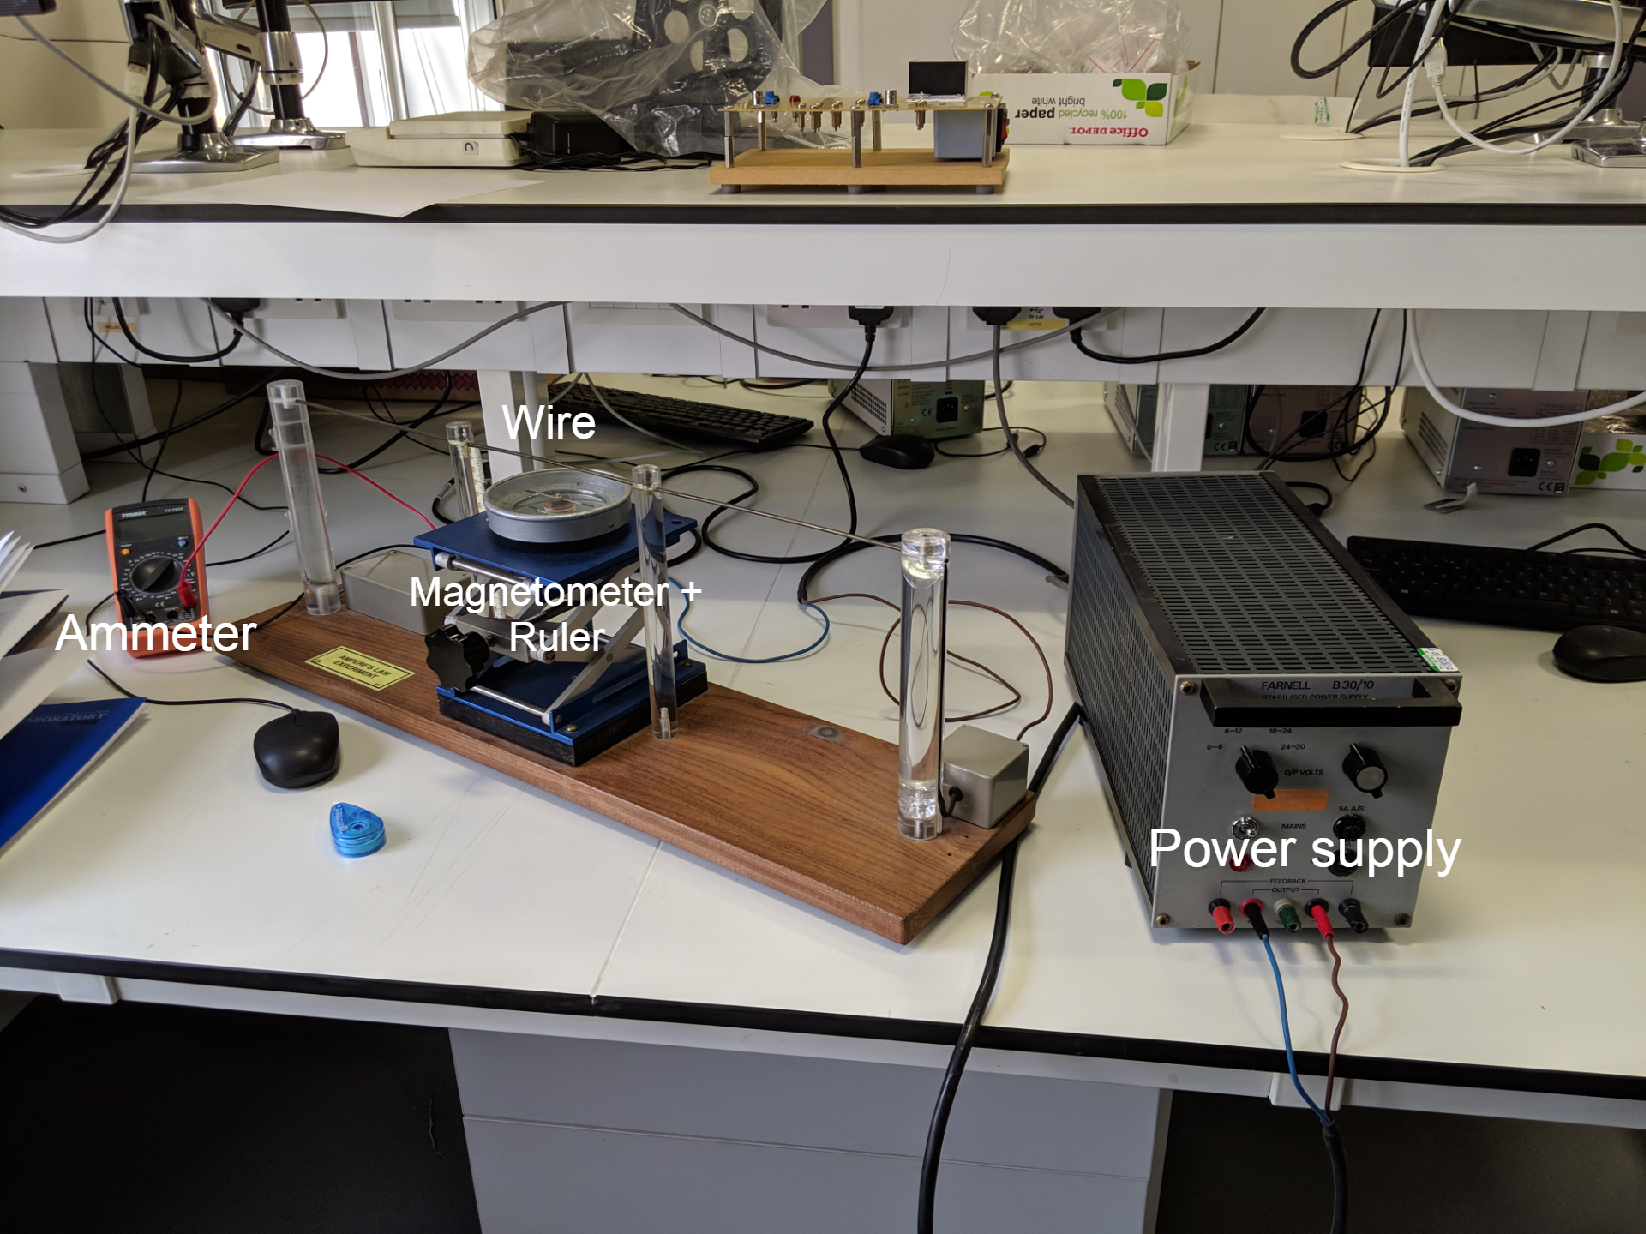
\includegraphics[width=\linewidth]{./img/apparatus.pdf}
  \caption{The apparatus}
  \label{fig:apparatus}
\end{figure}

It consists of the following components:

\begin{itemize}
  \item The wire
  \item An ammeter to measure the current
  \item The op amp/power supply
  \item Magnetometer with a ruler showing the distance from the wire
\end{itemize}

\subsection{Protocol}
\paragraph{}

The protocol is described below:

\begin{enumerate}
  \item Set the magnetometer so that the magnet (short needles) is parallel to the wire.
  \item Main loop using grid mesh(I:[2,3,4,5,6] [A] R:[2,3,4,5,6] [cm])
    \begin{enumerate}
      \item Set the current to I and distance of magnetometer to R.
      \item Measure the angular displacement \(\Phi\).
    \end{enumerate}
\end{enumerate}

\section{Results}
\paragraph{}

Our results are shown in Table \ref{tb:i} and Table \ref{tb:r}. Table \ref{tb:i} shows the results for when the current was changed with a constant value for \(R\) using 4 different values of \(R\). Table \ref{tb:r} shows the results for when the distance \(R\) was changed over 4 different constant currents.

\begin{table}[H]
\begin{tabular}{|l|l|l|l|l|l|}
\hline
R {[}m{]} & 1/R {[}1/m{]} & I {[}A{]} & \(\Phi\) {[}deg{]} & \(\tan{\Phi}\)        & BI {[}H{]} \\ \hline
2.00E-02  & 5.00E+01      & 5.04E+00  & 64          & 2.050303842 & 5.04E-05   \\ \hline
3.00E-02  & 3.33E+01      & 5.04E+00  & 59          & 1.664279482 & 3.36E-05   \\ \hline
4.00E-02  & 2.50E+01      & 5.04E+00  & 53          & 1.327044822 & 2.52E-05   \\ \hline
5.00E-02  & 2.00E+01      & 5.04E+00  & 46          & 1.035530314 & 2.02E-05   \\ \hline
6.00E-02  & 1.67E+01      & 5.04E+00  & 43          & 0.932515086 & 1.68E-05   \\ \hline
          &               &           &             &             &            \\ \hline
2.00E-02  & 5.00E+01      & 4.06E+00  & 59          & 1.664279482 & 4.06E-05   \\ \hline
3.00E-02  & 3.33E+01      & 4.06E+00  & 53          & 1.327044822 & 2.71E-05   \\ \hline
4.00E-02  & 2.50E+01      & 4.06E+00  & 47          & 1.07236871  & 2.03E-05   \\ \hline
5.00E-02  & 2.00E+01      & 4.06E+00  & 40          & 0.839099631 & 1.62E-05   \\ \hline
6.00E-02  & 1.67E+01      & 4.06E+00  & 36          & 0.726542528 & 1.35E-05   \\ \hline
          &               &           &             &             &            \\ \hline
2.00E-02  & 5.00E+01      & 3.07E+00  & 52          & 1.279941632 & 3.07E-05   \\ \hline
3.00E-02  & 3.33E+01      & 3.07E+00  & 45          & 1           & 2.05E-05   \\ \hline
4.00E-02  & 2.50E+01      & 3.07E+00  & 39          & 0.809784033 & 1.54E-05   \\ \hline
5.00E-02  & 2.00E+01      & 3.12E+00  & 33          & 0.649407593 & 1.25E-05   \\ \hline
6.00E-02  & 1.67E+01      & 3.10E+00  & 28          & 0.531709432 & 1.03E-05   \\ \hline
          &               &           &             &             &            \\ \hline
2.00E-02  & 5.00E+01      & 2.01E+00  & 40          & 0.839099631 & 2.01E-05   \\ \hline
3.00E-02  & 3.33E+01      & 2.01E+00  & 34          & 0.674508517 & 1.34E-05   \\ \hline
4.00E-02  & 2.50E+01      & 2.01E+00  & 27          & 0.509525449 & 1.01E-05   \\ \hline
5.00E-02  & 2.00E+01      & 2.01E+00  & 21          & 0.383864035 & 8.04E-06   \\ \hline
6.00E-02  & 1.67E+01      & 2.01E+00  & 18          & 0.324919696 & 6.70E-06   \\ \hline
\end{tabular}
\caption{Different values of \(R\) for constant values of \(I\)}
\label{tb:r}
\end{table}

\begin{table}[H]
\begin{tabular}{|l|l|l|l|l|}
\hline
R {[}m{]} & I {[}A{]} & \(\Phi\) {[}deg{]} & \(\tan{\Phi}\)        & BI {[}H{]} \\ \hline
2.00E-02  & 2.05E+00  & 48          & 1.110612515 & 2.05E-05   \\ \hline
2.00E-02  & 3.01E+00  & 53          & 1.327044822 & 3.01E-05   \\ \hline
2.00E-02  & 4.05E+00  & 60          & 1.732050808 & 4.05E-05   \\ \hline
2.00E-02  & 5.18E+00  & 65          & 2.144506921 & 5.18E-05   \\ \hline
2.00E-02  & 6.05E+00  & 68          & 2.475086853 & 6.05E-05   \\ \hline
          &           &             &             &            \\ \hline
3.00E-02  & 2.05E+00  & 35          & 0.700207538 & 1.37E-05   \\ \hline
3.00E-02  & 2.99E+00  & 45          & 1           & 1.99E-05   \\ \hline
3.00E-02  & 4.09E+00  & 54          & 1.37638192  & 2.73E-05   \\ \hline
3.00E-02  & 5.15E+00  & 59.5        & 1.697663119 & 3.43E-05   \\ \hline
3.00E-02  & 5.94E+00  & 63          & 1.962610506 & 3.96E-05   \\ \hline
          &           &             &             &            \\ \hline
4.00E-02  & 2.03E+00  & 28.5        & 0.5429557   & 1.02E-05   \\ \hline
4.00E-02  & 3.11E+00  & 40          & 0.839099631 & 1.56E-05   \\ \hline
4.00E-02  & 4.00E+00  & 47          & 1.07236871  & 2.00E-05   \\ \hline
4.00E-02  & 5.04E+00  & 53          & 1.327044822 & 2.52E-05   \\ \hline
4.00E-02  & 6.06E+00  & 58.5        & 1.631851687 & 3.03E-05   \\ \hline
          &           &             &             &            \\ \hline
5.00E-02  & 2.02E+00  & 15          & 0.267949192 & 8.08E-06   \\ \hline
5.00E-02  & 3.13E+00  & 33          & 0.649407593 & 1.25E-05   \\ \hline
5.00E-02  & 4.00E+00  & 40          & 0.839099631 & 1.60E-05   \\ \hline
5.00E-02  & 4.98E+00  & 46          & 1.035530314 & 1.99E-05   \\ \hline
5.00E-02  & 5.96E+00  & 52          & 1.279941632 & 2.38E-05   \\ \hline
\end{tabular}
\caption{Different values of \(I\) for constant \(R\)}
\label{tb:i}
\end{table}

The correlation between the current and distances with the tangent of the angular displacement are shown in Graphs \ref{g:i} and \ref{g:r}.

\begin{graph}[H]
  \includegraphics[width=\linewidth]{img/graph_i.pdf}
  \caption{Tangent of displacement over Current}
  \label{g:i}
\end{graph}

\begin{graph}[H]
  \includegraphics[width=\linewidth]{img/graph_r.pdf}
  \caption{Tangent of displacement over distance from wire}
  \label{g:r}
\end{graph}

\section{Uncertainty Analysis}
\paragraph{}

Combining \eqref{angle} and \eqref{flux_wire} we can deduce the following equation for \(B_E\).

\begin{equation}\label{flux_earth}
  B_E = 2\times10^{-7} \frac{I}{\tan{\Phi}R}
\end{equation}

Plugging the respective values into the equation and taking the average, we get the following value for the flux density of the Earth's magnetic field:

\[
  24.47 \pm 6.73 ~[\mu T]
\]

The random error was calculated in the following way;

\[ \Delta B_E = \frac{B_Emax - B_Emin}{2}\]

\section{Discussion and Conclusion}
\paragraph{}
The measured value of \(B_E\) does align with the known true value of \(B_E\) from the NOAA calculator:

\[ B_E \approx 19 ~[\mu T]\]

One of the reasons for the random error being so high may be due to the equipment being mostly analog. The power supply was also very sensitive and did not allow us to control it very precisely. Another possible cause for this may be due to noisy interference from nearby electronic devices as well.

The op amp in the power supply has a low output resistance \autocite{UPCSE2018}. This is helpful in this experiment because having a low resistance means that less power is required to achieve the relatively high amount of current required for the experiment.
\begin{figure}[H]
  \includegraphics[width=\linewidth]{img/circuit.pdf}
  \caption{The circuit diagram depicting the relevant section of the wire as a resistor}
  \label{fig:circ}
\end{figure}

\printbibliography
\end{document}
